\documentclass[12pt]{article} % -- letter, article, report, book, memoir



\usepackage{amsmath}
\usepackage{amssymb}
\usepackage{tikz}
\usepackage{graphicx}
\usepackage{hyperref}
\usepackage{wrapfig}
\usepackage{physics}
%=====linear algebra and general math notations
\newcommand{\rr}{\mathbb{R}}
\newcommand{\zz}{\mathbb{Z}}
\newcommand{\nn}{\mathbb{N}}
\newcommand{\cc}{\mathbb{C}}
\newcommand{\re}{\mathrm{Re}}
\newcommand{\im}{\mathrm{Im}}
\newcommand{\infnorm}[1]{\norm{#1}_{\infty}}
\newcommand{\twonorm}[1]{\norm{#1}_{2}}
\newcommand{\onenorm}[1]{\norm{#1}_{1}}
\newcommand{\iprod}[1]{\langle #1 \rangle}
\newcommand{\generalmatrixA}{
	\begin{pmatrix}
		a_{11} & a_{12} & \cdots & a_{1n} \\
		a_{21} & a_{22} & \cdots & a_{2n} \\
		\vdots & \vdots & \ddots & \vdots \\
		a_{n1} & a_{n2} & \cdots & a_{nn} \\
	\end{pmatrix}
}
%=====
%===== probability theory and random processes
\newcommand{\expect}[1]{\mathbb{E}\big[ {#1} \big]}
\newcommand{\cov}[1]{\mathbb{C}ov({#1})}
\newcommand{\pp}[1]{\mathbb{P}({#1})}
\newcommand{\variance}[1]{\mathbb{V}ar\big[{#1}\big]}
%=====
%===== PDE theory
\newcommand{\intervoo}[2]{(#1, #2)}
\newcommand{\intervcc}[2]{\big[ #1, #2\big]}
\newcommand{\pdx}[2]{\frac{\partial {#2}}{\partial {#1}}}
\newcommand{\pddx}[2]{\frac{\partial^2 {#2}}{\partial {#1}^2}}
\newcommand{\uno}{\large \textcircled{\small{1}}}
\newcommand{\dos}{\large\textcircled{\small{2}}}
\newcommand{\tres}{\large\textcircled{\small{3}}}
\newcommand{\yonn}{\large\textcircled{\small{4}}} % 4 in Japanese
\newcommand{\cancels}[1]{\underbrace{#1}_\textrm{cancelled}}
\newcommand{\ka}{\kappa}
\newcommand{\ga}{\gamma}
\newcommand{\uu}[2]{U_{#1}^{#2}} % shorthand
%=====
% ----------
\author{Hongli Zhao}
\title{Math 228B: Project 3 Writeup}
\date{\today}

\begin{document}
\maketitle
% ================ start file
\section{Burger's Equation Riemann Problem Linear Upwind Method}
We have the quasilinear Burger's equation:
$$
	u_t + uu_x = 0
$$

\subsection{(a) Find exact solution}
Due to the presence of jump discontinuities, the exact solution is in the Rankine-Hugoniot weak sense.
\subsubsection{initial condition $u_L < u_R$}
Using the method of characteristics, define:
$$
	\frac{dx(t)}{dt} = u(x(t),t)
$$ as our characteristic lines, by total derivative formula, solution $u$ is constant along the characteristics:
$$
	\frac{du}{dt} = \pdx{t}u + \pdx{x}u \frac{dx}{dt} = u_t + uu_x = 0
$$ thus the characteristic lines will be given by:
$$
	x(t) = u_0(x_0)t + x_0
$$ then given the initial data:
$$
	u(x,0) = \begin{cases}
		u_L = 0, x<0 \\
		u_R = 1, x>0
	\end{cases}
$$ we have that if $x_0 < 0$, $u_0(x_0) = 0$, and if $x_0 > 0$, $u_0(x_0) = 1$. Concisely:
$$
	x(t) = 
	\begin{cases}
		x_0, x_0 < 0 \\
		t + x_0, x_0 > 0
	\end{cases}
$$

In the $t-x$ plane, this is reflected as straight vertical lines on the left half of the plane, and straight lines of slope 1 on the right half of the plane. The region spanning $x = 0$ and $x = t$ is undefined. An infinite number of weak solutions can be defined. The two typical solutions are:

1. shock wave solution;
$$
	u(x,t) = 
	\begin{cases}
		0, x < st \\
		1, x>st
	\end{cases} 
$$ where $s$ is the speed of propagation.

In the shock wave solution, by the Rankine-Hugoniot condition, we have:
$$
	s(u_L - u_R) = f(u_L) = f(u_R)
$$ where $f$ is the quasilinear term.
$$
	s = \frac{\frac{1}{2}\cdot 1^2 - \frac12 \cdot 0^2}{1-0} = \frac12
$$

Therefore the shock wave solution is:
$$
	u(x,t) = \begin{cases}
		0, x < \frac12 t \\
		1, x>\frac12 t
	\end{cases} 
$$

Another physical solution is the rarefaction wave:
$$
	u(x,t) = \begin{cases}
		0, x \le 0 \\
		\frac{x}{t}, 0 \le x < t\\
		1, x> t
	\end{cases} 
$$ which corresponds to vanishing viscosity. We should use the rarefaction wave solution be our true exact solution, as it satisfies the entropy condition and is physical.
\subsubsection{initial condition $u_L > u_R$}
With the initial data:
$$
	u_0(t) = 
	\begin{cases}
		u_L = 1 \\
		u_R = 0
	\end{cases}
$$

The characteristic curves are switched (in terms of left and right half plane) compared to the previous case above. Therefore there exists a unique shock wave solution:
$$
	u(x,t) =
	\begin{cases}
		1, x < \frac12 t \\
		0, x > \frac{1}{2}t
	\end{cases}
$$ where the shock wave speed is determined already by the Rankine-Hugoniot condition in (a1).


\subsection{(b) Numerical Solution}
The final solutions at $t = 0.8$ are as follows, using  the finest level of discretization ($N=240$).
\subsection{$u_L < u_R$}
In the case $u_L<u_R$, with the CFL condition less than 1, the numerical solution has a rarefaction wave behavior.

It is also interesting to see that if we use a CFL condition of exactly 1, we get a shock wave solution (which is unphysical), we will be treating the rarefaction wave solution as our true solution in the following parts.

\begin{figure}[h]
\caption{Numerical solution for $u_L<u_R$ at $T=0.8$}
\centering
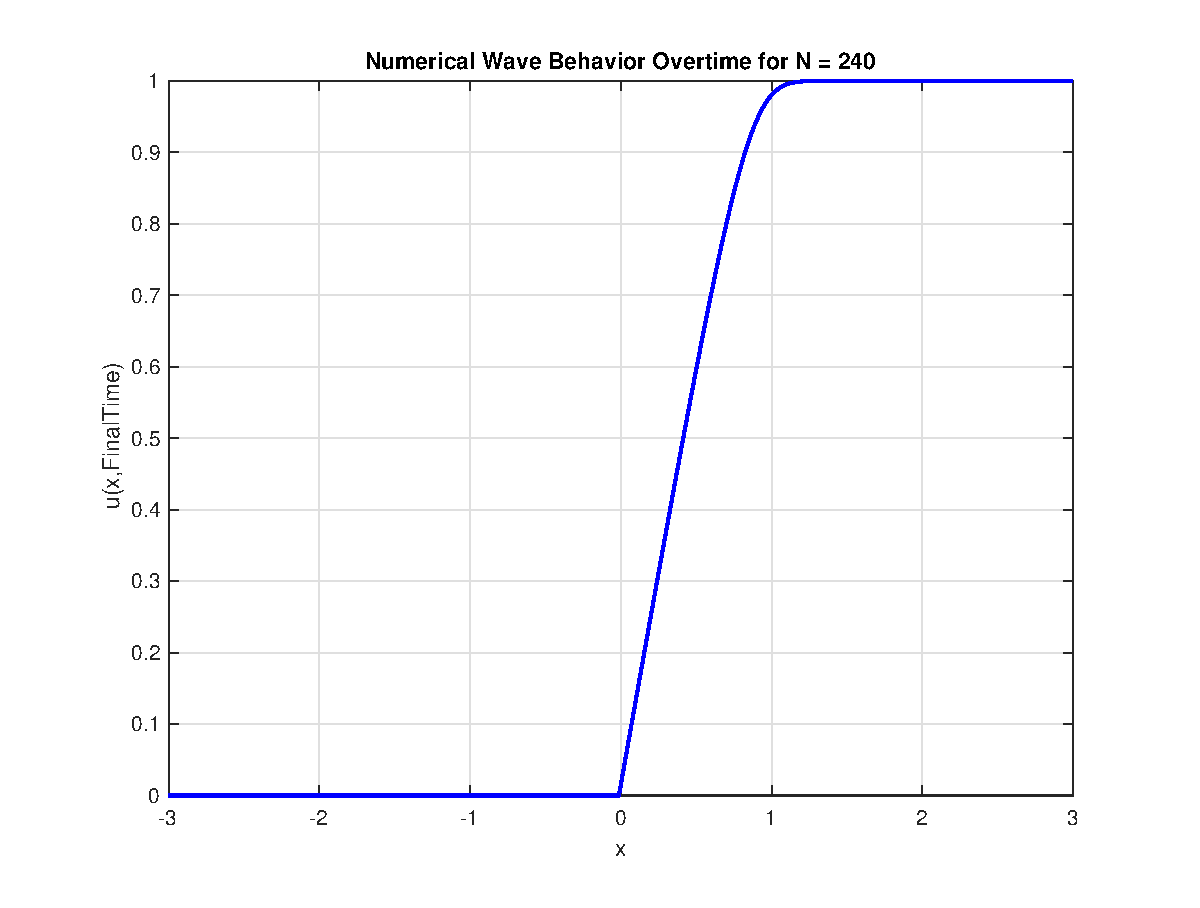
\includegraphics[width=0.65\textwidth]{p1b_1.eps}
\end{figure}


\begin{figure}[h]
\caption{Numerical solution for $u_L<u_R$, CFL=$1.0$, Shock wave behavior at $T=0.8$}
\centering
\includegraphics[width=0.65\textwidth]{right_shock.eps}
\end{figure}
\
\newpage
\
\
\newpage
\
\newpage
\subsection{$u_L > u_R$}
The numerical solution for this case is a jump discontinuity solution.

\begin{figure}[h]
\caption{Numerical solution for $u_L>u_R$ at $T=0.8$}
\centering
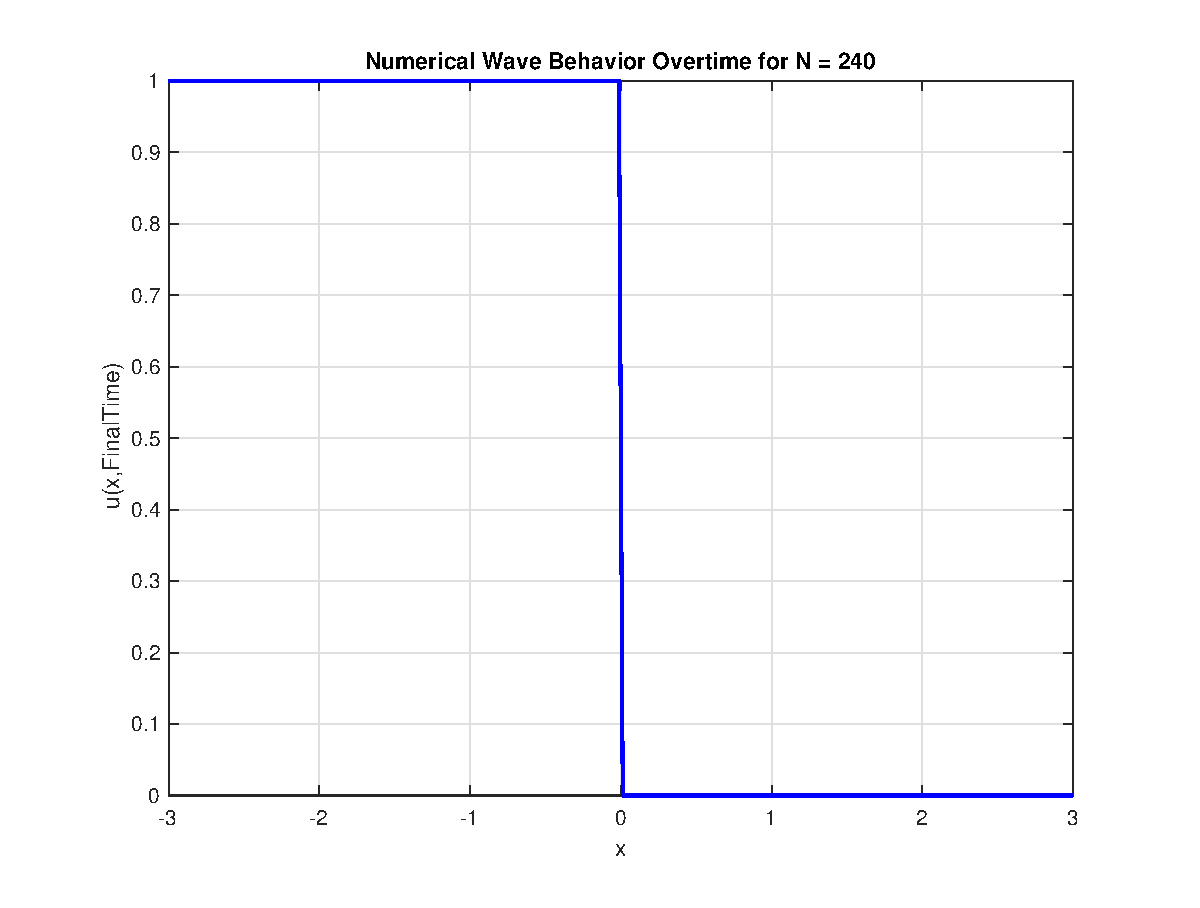
\includegraphics[width=0.65\textwidth]{p1b_2.eps}
\end{figure}


\subsection{(c) The CFL Condition}
We know for linear advection equation we have the form:
$$
	u_t + cu_x = 0
$$ yielding the CFL condition:
$$
	\abs{\frac{c\Delta x}{\Delta t}} \le 1
$$ via Von Neumann analysis.

In the nonlinear case, we can express the hyperbolic conservation law in quasilinear form:
$$
	u_t + u\cdot u_x = 0
$$ for the Burger's equation and use:
$$
	\abs{\frac{U_{max}\Delta x}{\Delta t}}\le 1
$$ as the CFL condition, where $U_{max}$ would be the maximum value of the numerical solution $U$ on the grid.

Since we always have $U_{j}^{n} \le 1$, we can let $U_{max} = 1$, and thus our CFL condition is:
$$
	\abs{\frac{\Delta t}{\Delta x}} \le 1
$$ which in the next section of this problem we show that different CFL conditions will give rise to different numerical behaviors.
\subsection{(d) Convergence of upwind method}
\subsection{$u_L < u_R$}
The log-log error plot (as a function of number of grid points $N$) is presented below. Since we are using $N = 240$ as the base solution, the error will become $0$ and log-log will be undefined at that point; therefore, we only plot $N=60,120$ and expect linear convergence. The error plot is overlaid with the $O(h)$ plot as a comparison.

\begin{figure}[h]
\caption{Log-Log Error Behavior $u_L<u_R$}
\centering
\includegraphics[width=0.65\textwidth]{1d_loglog.eps}
\end{figure}

The linear upwind scheme is (slightly better than) first order convergent.

\subsection{$u_L > u_R$}
Similarly, the log-log plot is:
\begin{figure}[h]
\caption{Log-Log Error Behavior $u_L>u_R$}
\centering
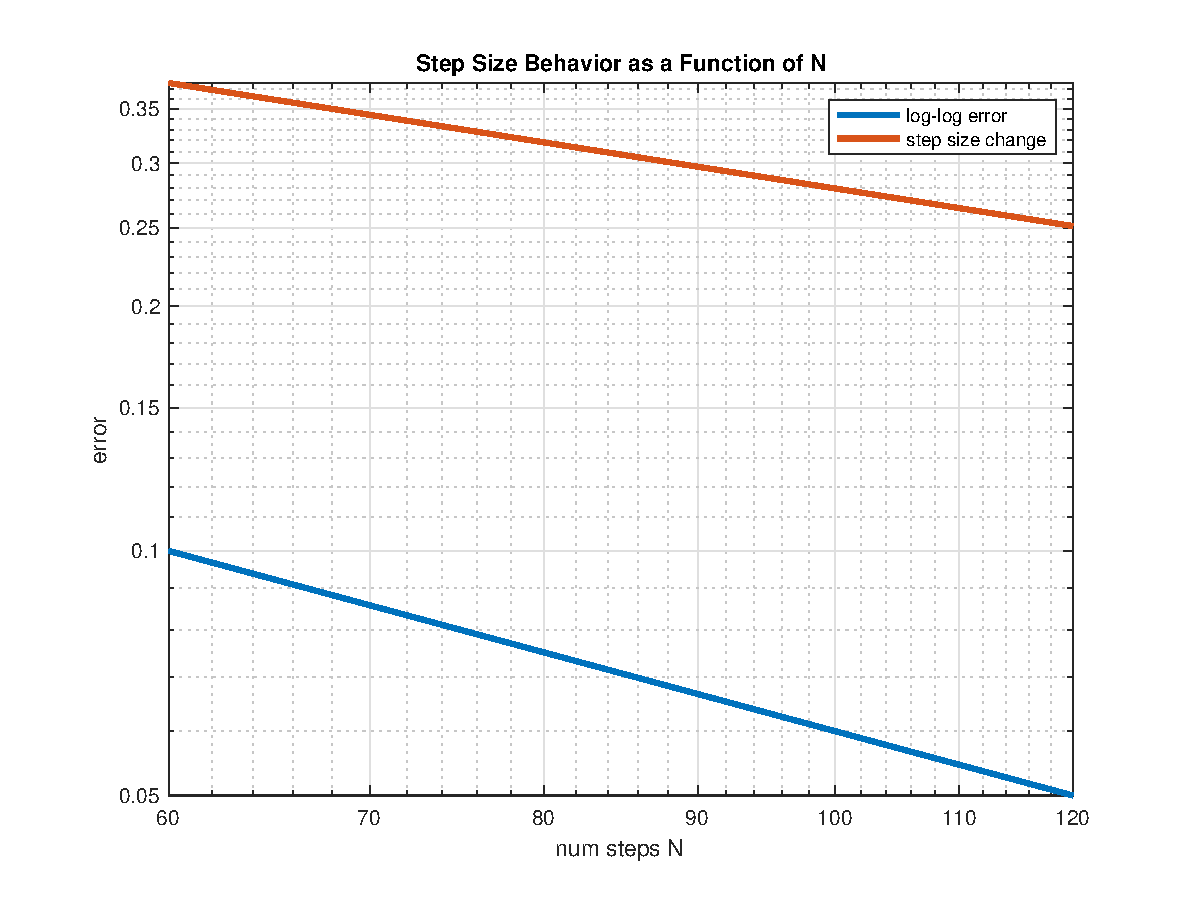
\includegraphics[width=0.65\textwidth]{1d_loglog2.eps}
\end{figure}

\subsection{(e)(f) Convergence}
\indent \indent As shown in the error plot, the method does converge as we increase the number of steps for our discretization. However, the method is not in conservative form, we would expect that it does not capture the advection behavior fully, and therefore does not converge to the true exact solution, as the plot shown below demonstrates, comparing the numerical solution at $N = 240$ with the exact weak solution. 
\subsection{(g) Comparison with exact solution}
\indent \indent The wave behavior is as follows, using $N = 240$. The linear upwind scheme fails to capture the advection and introduces error, especially in the jump discontinuity solution:
\begin{figure}[h!]
\caption{Numerical v. Exact Solution, $u_L < u_R$, at $T = 0.8$}
\centering
\includegraphics[width=0.8\textwidth]{p1g_compare1.eps}
\end{figure}

\begin{figure}[h!]
\caption{Numerical v. Exact Solution, $u_L > u_R$, at $T = 0.8$}
\centering
\includegraphics[width=0.8\textwidth]{1g_upwind_compare.eps}
\end{figure}

%======= prob2
\
\newpage
\
\section{Burger's Equation Riemann Problem Conservative Upwind Method}
Derivation of the scheme is as follows. 

Instead of discretizing the nonlinear term in $x$, we maintain the quasilinear form and choose to discretize the flux $f$ directly:
$$
	u_t + (f(u))_x = 0
$$ here the flux function for the Burger's equation is:
$$
	f(u) = \frac12 u^2
$$
\subsection{(a) Numerical Flux Function}
The conservative form use numerical differencing with respect to the flux directly, and the form is given by:
$$
	U_{j}^{n+1} = 
	U_{j}^{n} - \frac{\Delta t}{\Delta x} \big[ F(U_{j-p}^{n}, \cdots, U_{j}^{n}, \cdots, 
	U_{j+q}^{n}) - 
	F(U_{j-p-1}, \cdots, U_{j+q-1})\big]
$$

Given the first order upwind method:
$$
	U_{j}^{n+1} = U_{j}^{n} - 
	\frac{\Delta t}{\Delta x} (f(U_{j}^{n}) - f(U_{j-1}^{n}))
$$ discretizing the flux term, we plug in the flux function:
$$
	U_{j}^{n+1} = U_{j}^{n} - 
	\frac{\Delta t}{\Delta x}(\frac12 (U_{j}^{n})^2 - \frac12 (U_{j-1}^{n})^2)
$$ which is in the conservative form.

Thus our numerical flux function is the same as the flux:
$$
	F(U_{j}^n) = \frac12 (U_j^n)^2
$$

\subsection{(b) Convergence study}
Similar to the case of linear upwind method, we plot log-log error behavior using $N = 60, 120$ (since we are using $N=240$ as our base solution, the error at $N=240$ will be 0 and log will be undefined).

The conservative form upwind method is still first-order accurate as we increase the number of grid points. 

\begin{figure}[h!]
\caption{Log-Log Error Behavior, $u_L < u_R$}
\centering
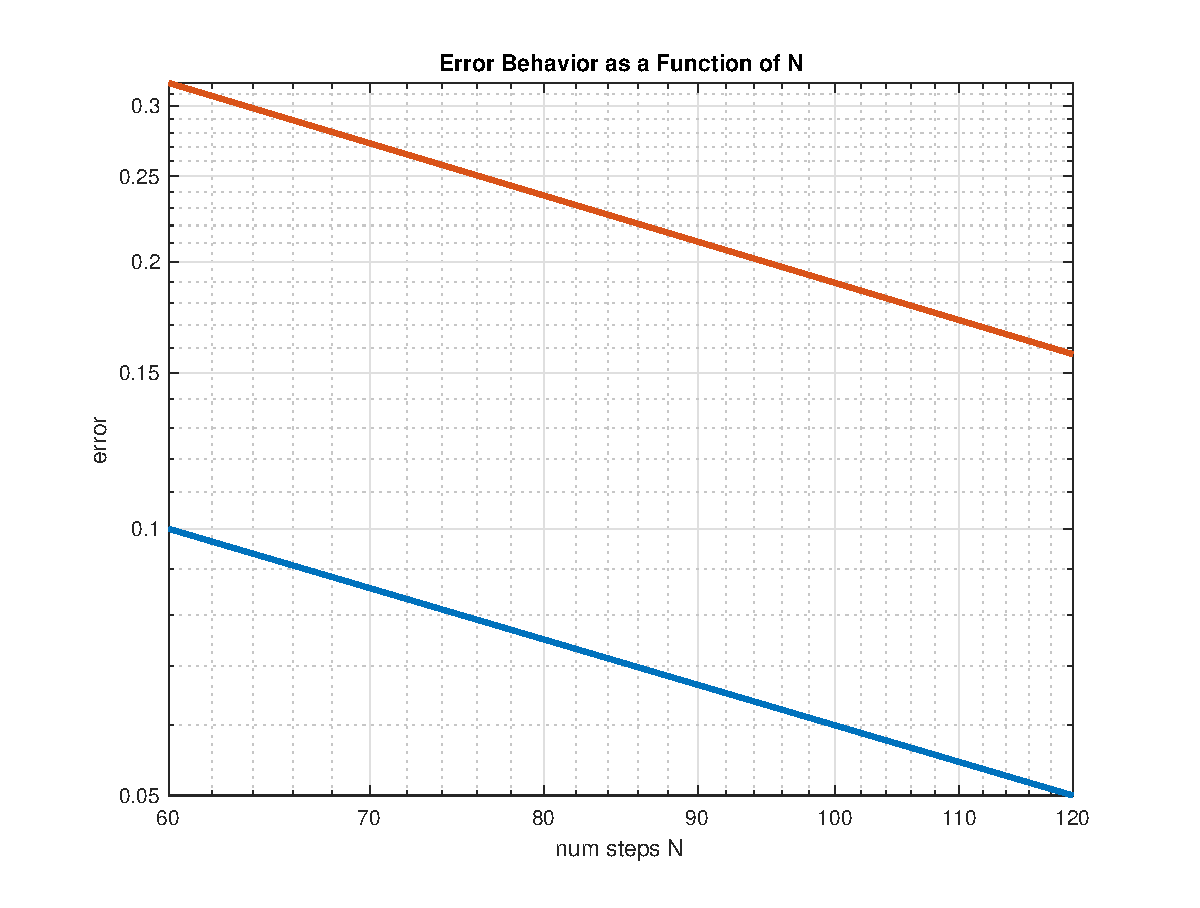
\includegraphics[width=0.65\textwidth]{converge1.eps}
\end{figure}

\begin{figure}[h!]
\caption{Log-Log Error Behavior, $u_L > u_R$}
\centering
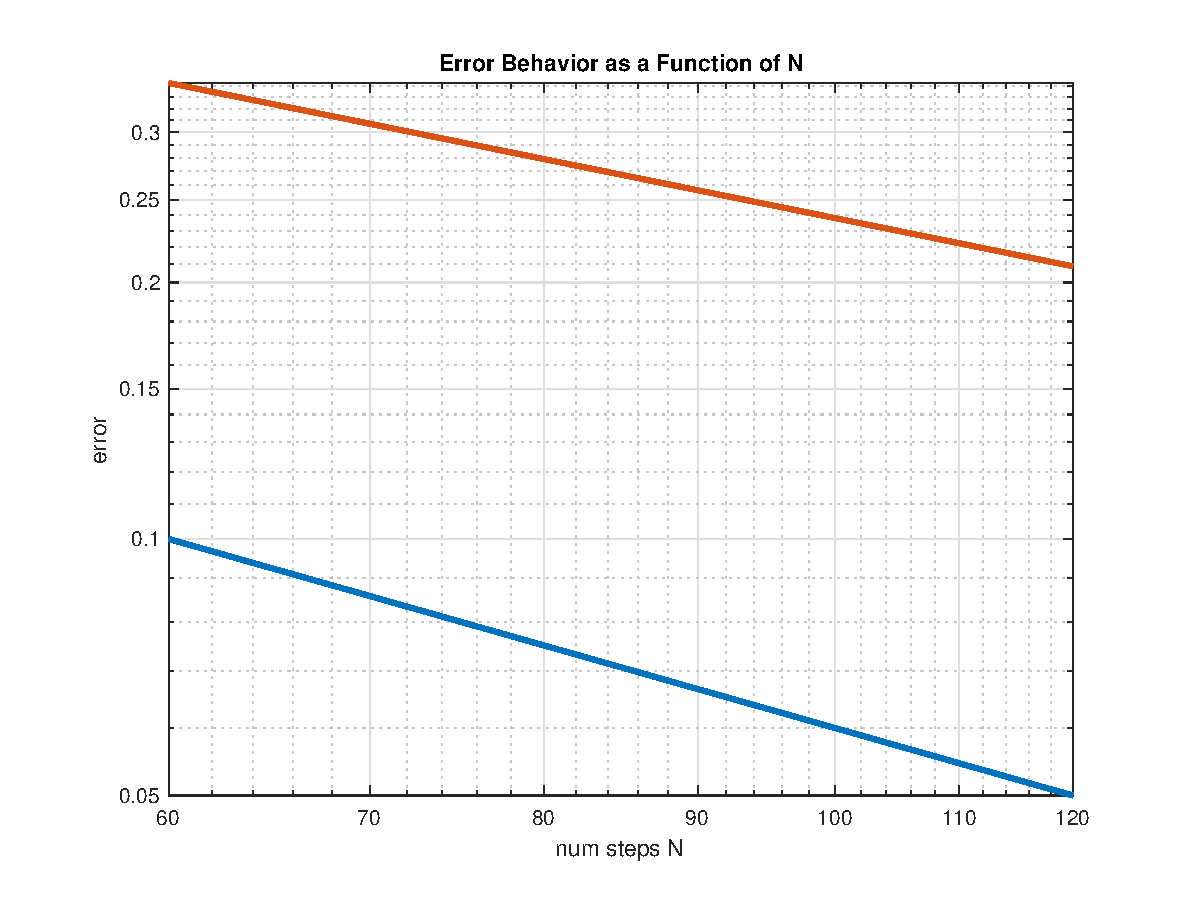
\includegraphics[width=0.65\textwidth]{converge2.eps}
\end{figure}
\newpage

\subsection{(c) Compare numerical solution with exact solution, superimposed plots}
The solution plots are presented below, at $T=0.8$ and with $N=240$.

\begin{figure}[h!]
\caption{Numerical v. Exact Solution, $u_L < u_R$, at $T = 0.8$}
\centering
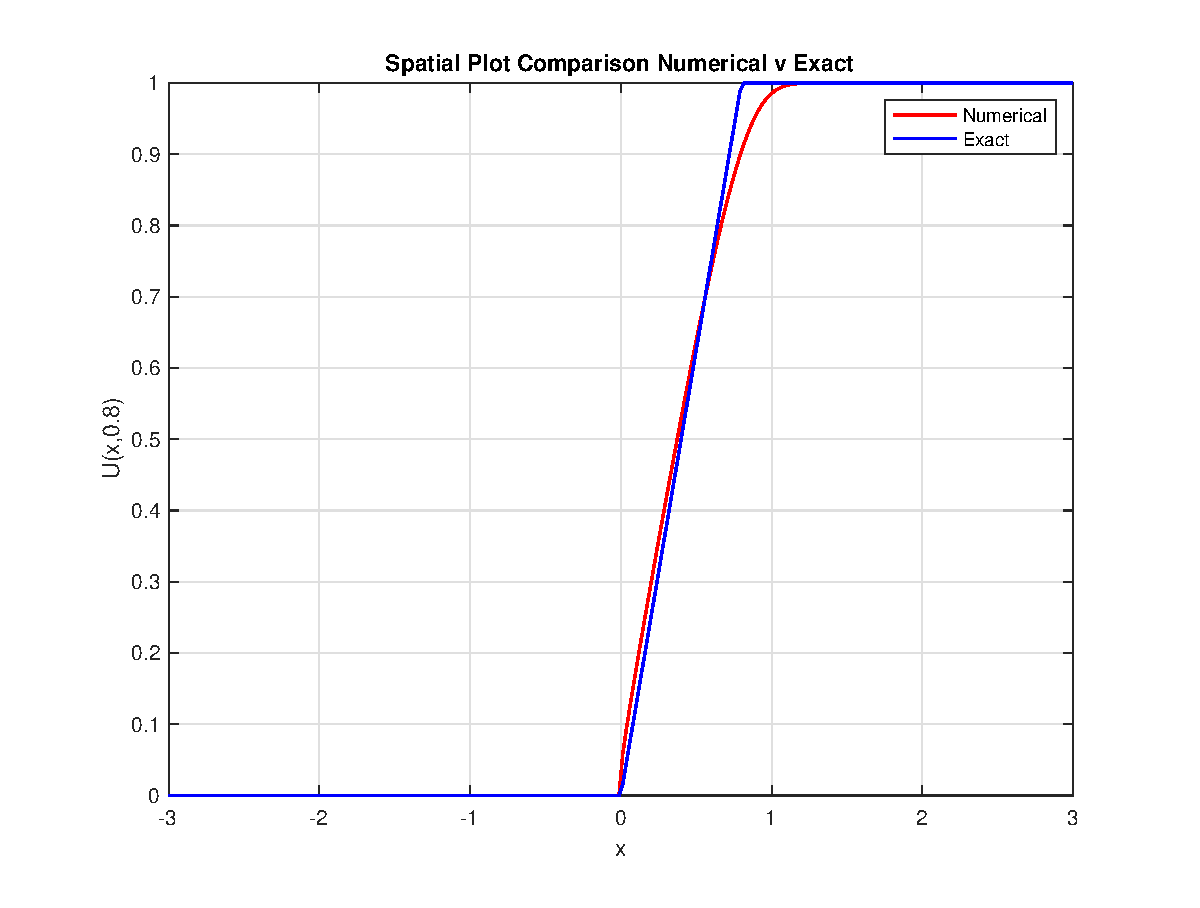
\includegraphics[width=0.8\textwidth]{compare2_2.eps}
\end{figure}

\begin{figure}[h!]
\caption{Numerical v. Exact Solution, $u_L > u_R$, at $T = 0.8$}
\centering
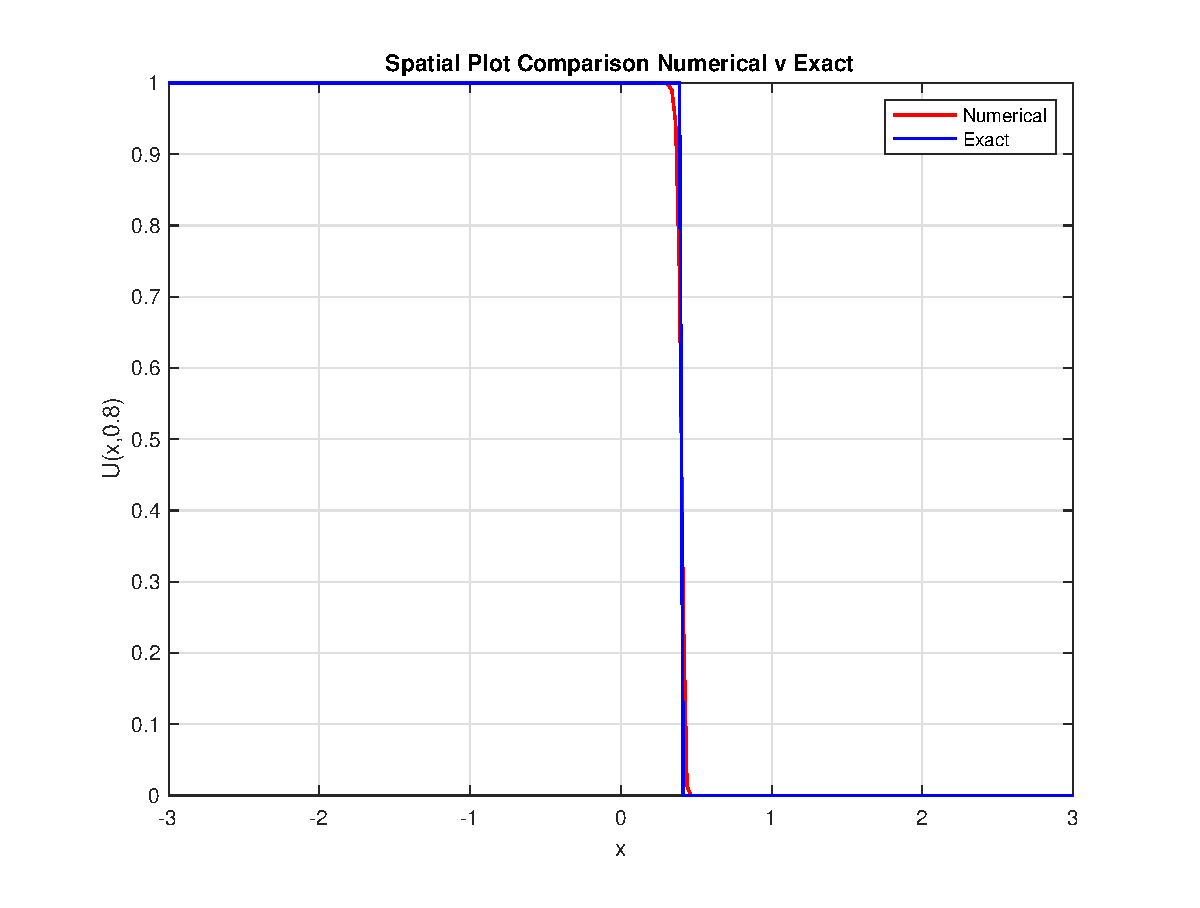
\includegraphics[width=0.8\textwidth]{compare2_1.eps}
\end{figure}

Although there are still errors present due to the method is only linearly accurate, we see that the conservative upwind method captures the advection of the jump discontinuity weak solution well.

\newpage
\subsection{(d) Point-wise differences between numerical and exact solution}
Absolute difference plot is also included. At time $T = 0.8$, using number of grid points $N = 240$:
\begin{figure}[h!]
\caption{Difference plot $u_L < u_R$, at $T = 0.8$}
\centering
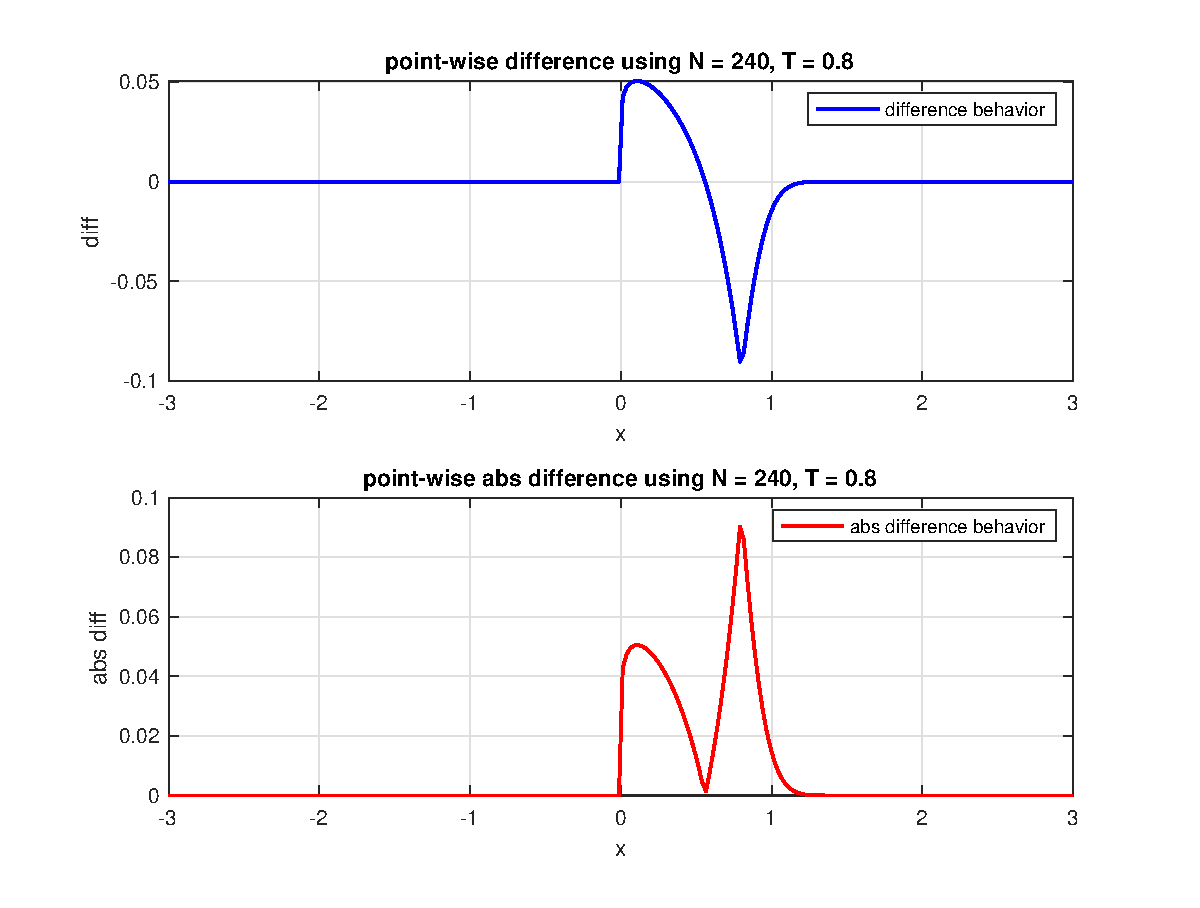
\includegraphics[width=0.8\textwidth]{diff1.eps}
\end{figure}

\begin{figure}[h!]
\caption{Difference plot $u_L > u_R$, at $T = 0.8$}
\centering
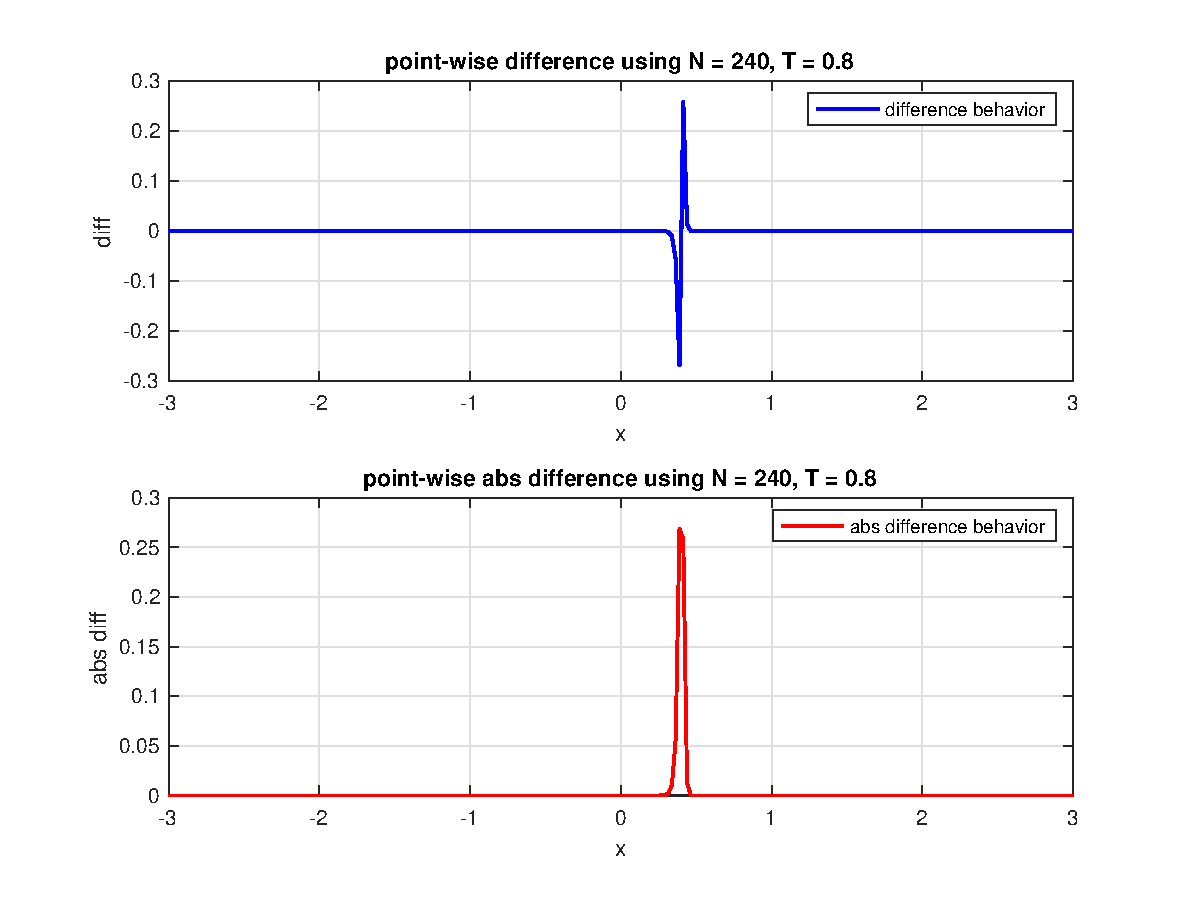
\includegraphics[width=0.8\textwidth]{diff2.eps}
\end{figure}

Looking at the difference plots and comparing them with the solution plots at $T = 0.8$ above, we see that errors tend to be large at the "sharp turns" of both solutions, when the solution transitions from one boundary to another.
\
\newpage
\
\section{Two Step Lax Wendroff with Strang Splitting}
Here we are solving the hyperbolic system:
$$
\begin{cases}
	\pdx{t}{A} + \pdx{x}{Q} = 0 \\
	\pdx{t}{Q} + \frac{\partial}{\partial x}(\alpha \frac{Q^2}{A}) + \frac{A}{\rho} \cdot \frac{\partial p(A)}{\partial x} = -2\cdot \frac{\alpha}{\alpha -1}\nu \frac{Q}{A}
\end{cases}
$$

With initial data:
$$
	\begin{pmatrix}
		A(x,0) \\
		Q(x,0)
	\end{pmatrix} = 
	\begin{pmatrix}
		A_0 \\
		0
	\end{pmatrix}
$$ and $A_0 > 0$.

And boundary data:
$$
	\begin{cases}
		p(0,t) = p_0(t)\\
		p(L,t) = p_L(t)
	\end{cases}
$$ with pressure function:
$$
	p(A) = G_0 (\sqrt{\frac{A}{A_0}}-1)
$$ and the derivative with respect to $A$ (useful in caculating the Jacobian below), is:
$$
	p'(A) = (\frac{G_0}{2\sqrt{A_0}})\frac{1}{\sqrt{A}}
$$	

The Lax-Wendroff scheme with Strang splitting is given. Let $h = \Delta x$ and $k = \Delta t$:
$$
	U_{j-\frac12}^{n+\frac12} = \frac12 (U_{j}^n + U_{j-1}^{n}) + \frac{1}{2}k\bigg[-\frac{F(U_{j}^n) - F(U_{j-1}^n)}{h} + \frac{S(U_{j}^{n}) - S(U_{j-1}^{n})}{2}\bigg]
$$
$$
	U_{j+\frac12}^{n+\frac12} = \frac12 (U_{j+1}^n + U_{j}) + \frac{1}{2}k\bigg[-\frac{F(U_{j+1}^n) - F(U_{j}^n)}{h} + \frac{S(U_{j+1}^{n}) - S(U_{j}^{n})}{2}\bigg]
$$
$$
	U_{j}^{n+1} = U_{j}^{n} - \frac{k}{h}
	\bigg[F(U_{j+\frac12}^{n+\frac12}) - F(U_{j-\frac12}^{n+\frac12})\bigg] + \frac{1}{2}k \bigg[S(U_{j+\frac12}^{n+\frac12}) - S(U_{j-\frac12}^{n+\frac12})\bigg]
$$ which is a 3-stencil.

\subsection{treating the boundary data}
At the boundaries, $x=0$ and $x=L$, we have the pressure information given by:
$$
	\begin{cases}
		p(0,t) = p_0(t)\\
		p(L,t) = p_{L}(t)
	\end{cases}
$$ using the pressure formula we can derive:
$$
	\begin{cases}
		p_0(t) = G_0(\sqrt{\frac{A(0,t)}{A_0}} - 1)\\
		p_{L}(t)= G_0(\sqrt{\frac{A(L,t)}{A_0}} - 1)
	\end{cases}
$$ and we have the boundary data for $A$:
$$
	\begin{cases}
		A(0,t) = A_0\bigg[\frac{1}{G_0}p_0(t) + 1\bigg]^2 \\
		A(L,t) = A_0\bigg[\frac{1}{G_0}p_L(t) + 1\bigg]^2
	\end{cases}
$$ 

At the boundaries, we would also need the data $Q(0,t), Q(L,t)$. To derive the data, we need to linearize the solution next to the boundaries, i.e. $U(1,t), U(L-h,t)$ and use "upwinding".

Linearization around a the solution $U_{*} = \begin{pmatrix}	A_{*} \\ Q_{*}\end{pmatrix}$ would yield:
\begin{equation}\label{eq:linearize}
	\begin{pmatrix}
		 A \\
		 Q
	\end{pmatrix}_{t}
	+
	\begin{pmatrix}
		 0 & 1 \\
		 -\alpha\frac{Q_{*}^2}{A_{*}^2}+\frac{1}{\rho} A_{*}p'(A_{*}) & 2\alpha\frac{Q_{*}}{A_{*}}
	\end{pmatrix} \cdot 
	\begin{pmatrix}
		 A \\
		 Q
	\end{pmatrix}_{x}
	= S(A,Q) = 
	\begin{pmatrix}
		 0 \\
		 f(A,Q)
	\end{pmatrix}
\end{equation} where $f$ is given by:
$$
	f(A,Q) = -2\frac{\alpha}{\alpha -1}\nu \frac{Q}{A}
$$

Letting $B$ to denote the Jacobian matrix in \eqref{eq:linearize}, the solution $U_{*}$ would approximate the boundary data well as $\Delta x,\Delta t$ become small. We can use the linearization and solve a linear system in the Riemann invariants, name $w_{*}, v_{*}$, which are functions of $Q,A$ (would like to recover $w_0^{n+1}, v_{N}^{n+1}$, from:
$$
	\begin{cases}
		w_t + \lambda_1^{*} w_x = s_1(w,v) \\
		v_t + \lambda_2^{*} v_x = s_2(w,v)
	\end{cases}
$$ where $\lambda^{*}$ is given by:
$$
	\lambda_{1,2} = \frac{\alpha Q}{A}\pm \sqrt{\alpha(\alpha-1)(\frac{Q}{A})^2 + \frac{G_0}{2\rho}(\frac{A}{A_0})^{\frac12}}
$$ with $\lambda_1 < \lambda_2$.

The system arose from diagonalizing the linerized system matrix $B$ above and finding the eigenvalues $\lambda_1,\lambda_2$. Then finding the left eigenvectors would yield a matrix $L = \begin{pmatrix}
	l_1^{T} \\
	l_2^{T}
\end{pmatrix}$ where $l_1,l_2$ are left eigenvectors. Then multiplying $L$ on both sides of the linearized hyperbolic system would yield:
$$
	L\begin{pmatrix}
		 A \\
		 Q
	\end{pmatrix}_{t}
	+
	\begin{pmatrix}
		 \lambda_1^{*} & 0 \\
		 0 & \lambda_2^{*}
	\end{pmatrix} \cdot 
	L\begin{pmatrix}
		 A \\
		 Q
	\end{pmatrix}_{x}
	= 
	L\begin{pmatrix}
		 0 \\
		 f(A,Q)
	\end{pmatrix} =
	\begin{pmatrix}
		 s_1 \\
		 s_2
	\end{pmatrix}
$$ then let $\begin{pmatrix}
		 w \\
		 v
	\end{pmatrix} = L
	\begin{pmatrix}
		 A \\
		 Q
	\end{pmatrix}$ gives us the system.

And use the upwind scheme to recover the boundary.

The upwind scheme is provided:
$$
	w_0^{n+1} = w_0^n - \frac{k}{h} \lambda_1^{*}(w_1^n - w_0^n) + \frac{k}{2} ((s_1)_1^n + (s_1)_0^n)
$$
$$
	v_N^{n+1} = v_{N}^n - \frac{k}{h} \lambda_2^{*}(v_N^{n} - v_{N-1}^{n}) + \frac{k}{2} ((s_2)_N^n + (s_2)_{N-1}^n)
$$

\subsection{Numerical results}
First, plot the velocity at midpoint for both the normal and hyperaemia cases. The MATLAB code takes $\sim 10$ minutes to run to fully complete the numerical solution.

At final time $0.763s \times 3 \text{ cycles} = 2.289 s$, the plots are as follows:
\begin{figure}[h!]
\caption{Profile, normal artery at final time, 3 cycles}
\centering
\includegraphics[width=1.0\textwidth]{normal4.eps}
\end{figure}

The midpoint velocity and cross-sectional area after stabilization is (1 cycle):
\begin{figure}[h!]
\caption{Velocity, Area and Flow profile, normal artery, 2 cycles}
\centering
\includegraphics[width=1.0\textwidth]{normal3.eps}
\end{figure}

The artery profile during hyperaemia is presented below, we see that the scheme is able to capture increased blood flow and velocity.
\begin{figure}[h!]
\caption{Profile, hyperaemia artery at final time, 3 cycles}
\centering
\includegraphics[width=1.0\textwidth]{hyper4.eps}
\end{figure}
\newpage
\begin{figure}[h!]
\caption{Velocity, Area and Flow profile, hyperaemia artery, 2 cycles}
\centering
\includegraphics[width=1.0\textwidth]{hyper3.eps}
\end{figure}
\
\newpage
\
\subsection{Reporting Maximum Mid-point Flow Rate}
The outputs for the reporting routine is as follows, MATLAB code included in zip file:
\begin{verbatim}
==========*==========*==========*==========
normal artery
maxflow reporting ...
max flow= 13.2923
\end{verbatim}

\begin{verbatim}
==========*==========*==========*==========
hyperaemia artery
maxflow reporting ...
max flow= 21.0546
\end{verbatim}

Thus this also shows that the scheme is able to capture the increased flow rate.
\subsection{Comment on plot behavior during first cycle $t\in\big[ 0,0.8\big]$}
The solution velocity seems to be unstable during the first simulation of cardiac cycle, with random values oscillating around the starting point. For the rest artery case, velocity was even initially negative, which is unphysical. 

Inspecting the numerical cross-sectional area, $A$ seems to exhibit oscillatory behavior during the first cycle and at times grows irregularly. As shown below (modified plotting routines to show what happened during $(0,0.763)$):
\begin{figure}[h!]
\caption{Profile, normal artery, full 3 cycles}
\centering
\includegraphics[width=1.0\textwidth]{full1.eps}
\end{figure}

\begin{figure}[h!]
\caption{Profile, hyperaemia artery, full 3 cycles}
\centering
\includegraphics[width=1.0\textwidth]{full2.eps}
\end{figure}

As shown in the plots, our scheme introduces oscillations before it stabilizes. 

% ================ end file
\end{document}

